\documentclass[1p]{elsarticle_modified}
%\bibliographystyle{elsarticle-num}

%\usepackage[colorlinks]{hyperref}
%\usepackage{abbrmath_seonhwa} %\Abb, \Ascr, \Acal ,\Abf, \Afrak
\usepackage{amsfonts}
\usepackage{amssymb}
\usepackage{amsmath}
\usepackage{amsthm}
\usepackage{scalefnt}
\usepackage{amsbsy}
\usepackage{kotex}
\usepackage{caption}
\usepackage{subfig}
\usepackage{color}
\usepackage{graphicx}
\usepackage{xcolor} %% white, black, red, green, blue, cyan, magenta, yellow
\usepackage{float}
\usepackage{setspace}
\usepackage{hyperref}

\usepackage{tikz}
\usetikzlibrary{arrows}

\usepackage{multirow}
\usepackage{array} % fixed length table
\usepackage{hhline}

%%%%%%%%%%%%%%%%%%%%%
\makeatletter
\renewcommand*\env@matrix[1][\arraystretch]{%
	\edef\arraystretch{#1}%
	\hskip -\arraycolsep
	\let\@ifnextchar\new@ifnextchar
	\array{*\c@MaxMatrixCols c}}
\makeatother %https://tex.stackexchange.com/questions/14071/how-can-i-increase-the-line-spacing-in-a-matrix
%%%%%%%%%%%%%%%

\usepackage[normalem]{ulem}

\newcommand{\msout}[1]{\ifmmode\text{\sout{\ensuremath{#1}}}\else\sout{#1}\fi}
%SOURCE: \msout is \stkout macro in https://tex.stackexchange.com/questions/20609/strikeout-in-math-mode

\newcommand{\cancel}[1]{
	\ifmmode
	{\color{red}\msout{#1}}
	\else
	{\color{red}\sout{#1}}
	\fi
}

\newcommand{\add}[1]{
	{\color{blue}\uwave{#1}}
}

\newcommand{\replace}[2]{
	\ifmmode
	{\color{red}\msout{#1}}{\color{blue}\uwave{#2}}
	\else
	{\color{red}\sout{#1}}{\color{blue}\uwave{#2}}
	\fi
}

\newcommand{\Sol}{\mathcal{S}} %segment
\newcommand{\D}{D} %diagram
\newcommand{\A}{\mathcal{A}} %arc


%%%%%%%%%%%%%%%%%%%%%%%%%%%%%5 test

\def\sl{\operatorname{\textup{SL}}(2,\Cbb)}
\def\psl{\operatorname{\textup{PSL}}(2,\Cbb)}
\def\quan{\mkern 1mu \triangleright \mkern 1mu}

\theoremstyle{definition}
\newtheorem{thm}{Theorem}[section]
\newtheorem{prop}[thm]{Proposition}
\newtheorem{lem}[thm]{Lemma}
\newtheorem{ques}[thm]{Question}
\newtheorem{cor}[thm]{Corollary}
\newtheorem{defn}[thm]{Definition}
\newtheorem{exam}[thm]{Example}
\newtheorem{rmk}[thm]{Remark}
\newtheorem{alg}[thm]{Algorithm}

\newcommand{\I}{\sqrt{-1}}
\begin{document}

%\begin{frontmatter}
%
%\title{Boundary parabolic representations of knots up to 8 crossings}
%
%%% Group authors per affiliation:
%\author{Yunhi Cho} 
%\address{Department of Mathematics, University of Seoul, Seoul, Korea}
%\ead{yhcho@uos.ac.kr}
%
%
%\author{Seonhwa Kim} %\fnref{s_kim}}
%\address{Center for Geometry and Physics, Institute for Basic Science, Pohang, 37673, Korea}
%\ead{ryeona17@ibs.re.kr}
%
%\author{Hyuk Kim}
%\address{Department of Mathematical Sciences, Seoul National University, Seoul 08826, Korea}
%\ead{hyukkim@snu.ac.kr}
%
%\author{Seokbeom Yoon}
%\address{Department of Mathematical Sciences, Seoul National University, Seoul, 08826,  Korea}
%\ead{sbyoon15@snu.ac.kr}
%
%\begin{abstract}
%We find all boundary parabolic representation of knots up to 8 crossings.
%
%\end{abstract}
%\begin{keyword}
%    \MSC[2010] 57M25 
%\end{keyword}
%
%\end{frontmatter}

%\linenumbers
%\tableofcontents
%
\newcommand\colored[1]{\textcolor{white}{\rule[-0.35ex]{0.8em}{1.4ex}}\kern-0.8em\color{red} #1}%
%\newcommand\colored[1]{\textcolor{white}{ #1}\kern-2.17ex	\textcolor{white}{ #1}\kern-1.81ex	\textcolor{white}{ #1}\kern-2.15ex\color{red}#1	}

{\Large $\underline{12a_{1222}~(K12a_{1222})}$}

\setlength{\tabcolsep}{10pt}
\renewcommand{\arraystretch}{1.6}
\vspace{1cm}\begin{tabular}{m{100pt}>{\centering\arraybackslash}m{274pt}}
\multirow{5}{120pt}{
	\centering
	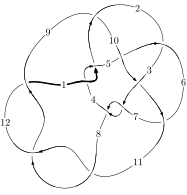
\includegraphics[width=112pt]{../../../GIT/diagram.site/Diagrams/png/2023_12a_1222.png}\\
\ \ \ A knot diagram\footnotemark}&
\allowdisplaybreaks
\textbf{Linearized knot diagam} \\
\cline{2-2}
 &
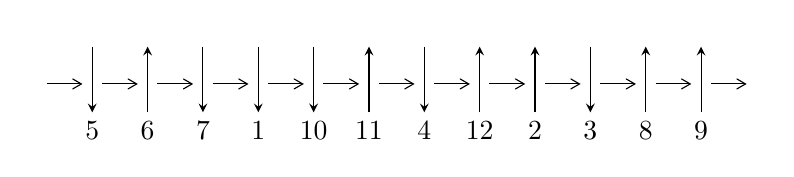
\begin{tikzpicture}[x=20pt, y=17pt]
	% nodes
	\node (C0) at (0, 0) {};
	\node (C1) at (1, 0) {};
	\node (C1U) at (1, +1) {};
	\node (C1D) at (1, -1) {5};

	\node (C2) at (2, 0) {};
	\node (C2U) at (2, +1) {};
	\node (C2D) at (2, -1) {6};

	\node (C3) at (3, 0) {};
	\node (C3U) at (3, +1) {};
	\node (C3D) at (3, -1) {7};

	\node (C4) at (4, 0) {};
	\node (C4U) at (4, +1) {};
	\node (C4D) at (4, -1) {1};

	\node (C5) at (5, 0) {};
	\node (C5U) at (5, +1) {};
	\node (C5D) at (5, -1) {10};

	\node (C6) at (6, 0) {};
	\node (C6U) at (6, +1) {};
	\node (C6D) at (6, -1) {11};

	\node (C7) at (7, 0) {};
	\node (C7U) at (7, +1) {};
	\node (C7D) at (7, -1) {4};

	\node (C8) at (8, 0) {};
	\node (C8U) at (8, +1) {};
	\node (C8D) at (8, -1) {12};

	\node (C9) at (9, 0) {};
	\node (C9U) at (9, +1) {};
	\node (C9D) at (9, -1) {2};

	\node (C10) at (10, 0) {};
	\node (C10U) at (10, +1) {};
	\node (C10D) at (10, -1) {3};

	\node (C11) at (11, 0) {};
	\node (C11U) at (11, +1) {};
	\node (C11D) at (11, -1) {8};

	\node (C12) at (12, 0) {};
	\node (C12U) at (12, +1) {};
	\node (C12D) at (12, -1) {9};
	\node (C13) at (13, 0) {};

	% arrows
	\draw[->,>={angle 60}]
	(C0) edge (C1) (C1) edge (C2) (C2) edge (C3) (C3) edge (C4) (C4) edge (C5) (C5) edge (C6) (C6) edge (C7) (C7) edge (C8) (C8) edge (C9) (C9) edge (C10) (C10) edge (C11) (C11) edge (C12) (C12) edge (C13) ;	\draw[->,>=stealth]
	(C1U) edge (C1D) (C2D) edge (C2U) (C3U) edge (C3D) (C4U) edge (C4D) (C5U) edge (C5D) (C6D) edge (C6U) (C7U) edge (C7D) (C8D) edge (C8U) (C9D) edge (C9U) (C10U) edge (C10D) (C11D) edge (C11U) (C12D) edge (C12U) ;
	\end{tikzpicture} \\
\hhline{~~} \\& 
\textbf{Solving Sequence} \\ \cline{2-2} 
 &
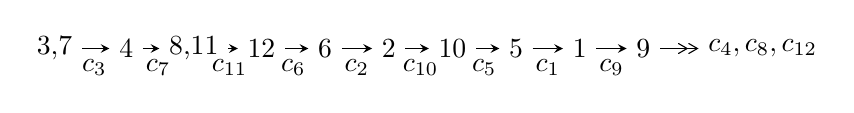
\begin{tikzpicture}[x=23pt, y=7pt]
	% node
	\node (A0) at (-1/8, 0) {3,7};
	\node (A1) at (1, 0) {4};
	\node (A2) at (33/16, 0) {8,11};
	\node (A3) at (25/8, 0) {12};
	\node (A4) at (33/8, 0) {6};
	\node (A5) at (41/8, 0) {2};
	\node (A6) at (49/8, 0) {10};
	\node (A7) at (57/8, 0) {5};
	\node (A8) at (65/8, 0) {1};
	\node (A9) at (73/8, 0) {9};
	\node (C1) at (1/2, -1) {$c_{3}$};
	\node (C2) at (3/2, -1) {$c_{7}$};
	\node (C3) at (21/8, -1) {$c_{11}$};
	\node (C4) at (29/8, -1) {$c_{6}$};
	\node (C5) at (37/8, -1) {$c_{2}$};
	\node (C6) at (45/8, -1) {$c_{10}$};
	\node (C7) at (53/8, -1) {$c_{5}$};
	\node (C8) at (61/8, -1) {$c_{1}$};
	\node (C9) at (69/8, -1) {$c_{9}$};
	\node (A10) at (11, 0) {$c_{4},c_{8},c_{12}$};

	% edge
	\draw[->,>=stealth]	
	(A0) edge (A1) (A1) edge (A2) (A2) edge (A3) (A3) edge (A4) (A4) edge (A5) (A5) edge (A6) (A6) edge (A7) (A7) edge (A8) (A8) edge (A9) ;
	\draw[->>,>={angle 60}]	
	(A9) edge (A10);
\end{tikzpicture} \\ 

\end{tabular} \\

\footnotetext{
The image of knot diagram is generated by the software ``\textbf{Draw programme}" developed by Andrew Bartholomew(\url{http://www.layer8.co.uk/maths/draw/index.htm\#Running-draw}), where we modified some parts for our purpose(\url{https://github.com/CATsTAILs/LinksPainter}).
}\phantom \\ \newline 
\centering \textbf{Ideals for irreducible components\footnotemark of $X_{\text{par}}$} 
 
\begin{align*}
I^u_{1}&=\langle 
8.54050\times10^{28} u^{33}-1.19908\times10^{29} u^{32}+\cdots+2.02956\times10^{29} b-1.46806\times10^{29},\\
\phantom{I^u_{1}}&\phantom{= \langle  }2.00324\times10^{28} u^{33}-1.85192\times10^{28} u^{32}+\cdots+1.19386\times10^{28} a-1.66365\times10^{29},\;u^{34}- u^{33}+\cdots-14 u+1\rangle \\
I^u_{2}&=\langle 
-1.00686\times10^{316} u^{83}-2.20932\times10^{316} u^{82}+\cdots+1.65013\times10^{317} b-2.02613\times10^{318},\\
\phantom{I^u_{2}}&\phantom{= \langle  }3.54486\times10^{318} u^{83}+6.01988\times10^{318} u^{82}+\cdots+3.48177\times10^{319} a-5.74769\times10^{319},\\
\phantom{I^u_{2}}&\phantom{= \langle  }u^{84}+3 u^{83}+\cdots+1498 u+211\rangle \\
I^u_{3}&=\langle 
u^{11}+u^{10}-5 u^9- u^8+12 u^7-3 u^6-20 u^5+9 u^4+17 u^3-12 u^2+b-8 u+5,\\
\phantom{I^u_{3}}&\phantom{= \langle  }6 u^{11}-3 u^{10}-20 u^9+15 u^8+38 u^7-43 u^6-46 u^5+59 u^4+28 u^3-49 u^2+a-11 u+14,\\
\phantom{I^u_{3}}&\phantom{= \langle  }u^{12}- u^{11}-3 u^{10}+4 u^9+5 u^8-10 u^7-4 u^6+13 u^5-10 u^3+2 u^2+3 u-1\rangle \\
I^u_{4}&=\langle 
b-1,\;a-1,\;u^2+u-1\rangle \\
I^u_{5}&=\langle 
b- u,\;a- u-1,\;u^2+u-1\rangle \\
\\
\end{align*}
\raggedright * 5 irreducible components of $\dim_{\mathbb{C}}=0$, with total 134 representations.\\
\footnotetext{All coefficients of polynomials are rational numbers. But the coefficients are sometimes approximated in decimal forms when there is not enough margin.}
\newpage
\renewcommand{\arraystretch}{1}
\centering \section*{I. $I^u_{1}= \langle 8.54\times10^{28} u^{33}-1.20\times10^{29} u^{32}+\cdots+2.03\times10^{29} b-1.47\times10^{29},\;2.00\times10^{28} u^{33}-1.85\times10^{28} u^{32}+\cdots+1.19\times10^{28} a-1.66\times10^{29},\;u^{34}- u^{33}+\cdots-14 u+1 \rangle$}
\flushleft \textbf{(i) Arc colorings}\\
\begin{tabular}{m{7pt} m{180pt} m{7pt} m{180pt} }
\flushright $a_{3}=$&$\begin{pmatrix}1\\0\end{pmatrix}$ \\
\flushright $a_{7}=$&$\begin{pmatrix}0\\u\end{pmatrix}$ \\
\flushright $a_{4}=$&$\begin{pmatrix}1\\u^2\end{pmatrix}$ \\
\flushright $a_{8}=$&$\begin{pmatrix}- u\\- u^3+u\end{pmatrix}$ \\
\flushright $a_{11}=$&$\begin{pmatrix}-1.67795 u^{33}+1.55120 u^{32}+\cdots-54.4816 u+13.9351\\-0.420805 u^{33}+0.590807 u^{32}+\cdots+0.214756 u+0.723340\end{pmatrix}$ \\
\flushright $a_{12}=$&$\begin{pmatrix}-1.82607 u^{33}+1.79373 u^{32}+\cdots-55.2072 u+14.1232\\-0.374427 u^{33}+0.626344 u^{32}+\cdots+2.41017 u+0.440872\end{pmatrix}$ \\
\flushright $a_{6}=$&$\begin{pmatrix}0.0849368 u^{33}-0.674220 u^{32}+\cdots-22.0169 u-4.53343\\0.0652050 u^{33}-0.290176 u^{32}+\cdots-4.20788 u+0.0290844\end{pmatrix}$ \\
\flushright $a_{2}=$&$\begin{pmatrix}1.23819 u^{33}-1.28700 u^{32}+\cdots+25.7222 u+0.477757\\0.429517 u^{33}-0.646675 u^{32}+\cdots-0.921613 u+0.0488161\end{pmatrix}$ \\
\flushright $a_{10}=$&$\begin{pmatrix}-2.09876 u^{33}+2.14201 u^{32}+\cdots-54.2669 u+14.6584\\-0.420805 u^{33}+0.590807 u^{32}+\cdots+0.214756 u+0.723340\end{pmatrix}$ \\
\flushright $a_{5}=$&$\begin{pmatrix}1.11813 u^{33}-2.58902 u^{32}+\cdots-39.5230 u+1.70908\\1.06931 u^{33}-2.11069 u^{32}+\cdots-21.7107 u+1.47090\end{pmatrix}$ \\
\flushright $a_{1}=$&$\begin{pmatrix}2.70908 u^{33}-3.82721 u^{32}+\cdots+8.35933 u+1.59588\\1.47090 u^{33}-2.54021 u^{32}+\cdots-17.3628 u+1.11813\end{pmatrix}$ \\
\flushright $a_{9}=$&$\begin{pmatrix}-0.370824 u^{33}+1.27805 u^{32}+\cdots+28.8631 u+4.34212\\-0.628147 u^{33}+1.22765 u^{32}+\cdots+14.1089 u-0.498700\end{pmatrix}$\\&\end{tabular}
\flushleft \textbf{(ii) Obstruction class $= -1$}\\~\\
\flushleft \textbf{(iii) Cusp Shapes $= 2.52397 u^{33}-1.46607 u^{32}+\cdots+104.427 u-1.38626$}\\~\\
\newpage\renewcommand{\arraystretch}{1}
\flushleft \textbf{(iv) u-Polynomials at the component}\newline \\
\begin{tabular}{m{50pt}|m{274pt}}
Crossings & \hspace{64pt}u-Polynomials at each crossing \\
\hline $$\begin{aligned}c_{1},c_{3},c_{4}\\c_{7}\end{aligned}$$&$\begin{aligned}
&u^{34}- u^{33}+\cdots-14 u+1
\end{aligned}$\\
\hline $$\begin{aligned}c_{2}\end{aligned}$$&$\begin{aligned}
&u^{34}-15 u^{33}+\cdots-42 u+4
\end{aligned}$\\
\hline $$\begin{aligned}c_{5},c_{10}\end{aligned}$$&$\begin{aligned}
&u^{34}- u^{33}+\cdots+2 u-1
\end{aligned}$\\
\hline $$\begin{aligned}c_{6},c_{9}\end{aligned}$$&$\begin{aligned}
&u^{34}- u^{33}+\cdots+8 u+1
\end{aligned}$\\
\hline $$\begin{aligned}c_{8},c_{11},c_{12}\end{aligned}$$&$\begin{aligned}
&u^{34}-12 u^{33}+\cdots+48 u+16
\end{aligned}$\\
\hline
\end{tabular}\\~\\
\newpage\renewcommand{\arraystretch}{1}
\flushleft \textbf{(v) Riley Polynomials at the component}\newline \\
\begin{tabular}{m{50pt}|m{274pt}}
Crossings & \hspace{64pt}Riley Polynomials at each crossing \\
\hline $$\begin{aligned}c_{1},c_{3},c_{4}\\c_{7}\end{aligned}$$&$\begin{aligned}
&y^{34}-29 y^{33}+\cdots-146 y+1
\end{aligned}$\\
\hline $$\begin{aligned}c_{2}\end{aligned}$$&$\begin{aligned}
&y^{34}-7 y^{33}+\cdots-1628 y+16
\end{aligned}$\\
\hline $$\begin{aligned}c_{5},c_{10}\end{aligned}$$&$\begin{aligned}
&y^{34}-23 y^{33}+\cdots-42 y+1
\end{aligned}$\\
\hline $$\begin{aligned}c_{6},c_{9}\end{aligned}$$&$\begin{aligned}
&y^{34}-5 y^{33}+\cdots-48 y+1
\end{aligned}$\\
\hline $$\begin{aligned}c_{8},c_{11},c_{12}\end{aligned}$$&$\begin{aligned}
&y^{34}-36 y^{33}+\cdots+480 y+256
\end{aligned}$\\
\hline
\end{tabular}\\~\\
\newpage\flushleft \textbf{(vi) Complex Volumes and Cusp Shapes}
$$\begin{array}{c|c|c}  
\text{Solutions to }I^u_{1}& \I (\text{vol} + \sqrt{-1}CS) & \text{Cusp shape}\\
 \hline 
\begin{aligned}
u &= \phantom{-}0.911688 + 0.363959 I \\
a &= -0.171944 + 0.102128 I \\
b &= \phantom{-}1.10685 - 1.31639 I\end{aligned}
 & \phantom{-}2.69872 - 3.21839 I & \phantom{-}4.59732 + 8.11808 I \\ \hline\begin{aligned}
u &= \phantom{-}0.911688 - 0.363959 I \\
a &= -0.171944 - 0.102128 I \\
b &= \phantom{-}1.10685 + 1.31639 I\end{aligned}
 & \phantom{-}2.69872 + 3.21839 I & \phantom{-}4.59732 - 8.11808 I \\ \hline\begin{aligned}
u &= -0.927431 + 0.304938 I \\
a &= \phantom{-}0.474616 - 0.316310 I \\
b &= -0.220232 + 0.174637 I\end{aligned}
 & -1.71183 + 0.63600 I & -2.75071 - 0.30580 I \\ \hline\begin{aligned}
u &= -0.927431 - 0.304938 I \\
a &= \phantom{-}0.474616 + 0.316310 I \\
b &= -0.220232 - 0.174637 I\end{aligned}
 & -1.71183 - 0.63600 I & -2.75071 + 0.30580 I \\ \hline\begin{aligned}
u &= \phantom{-}1.038620 + 0.229840 I \\
a &= \phantom{-}1.201340 + 0.604971 I \\
b &= \phantom{-}1.061670 + 0.056991 I\end{aligned}
 & -1.18415 - 2.37587 I & -5.06552 + 2.01648 I \\ \hline\begin{aligned}
u &= \phantom{-}1.038620 - 0.229840 I \\
a &= \phantom{-}1.201340 - 0.604971 I \\
b &= \phantom{-}1.061670 - 0.056991 I\end{aligned}
 & -1.18415 + 2.37587 I & -5.06552 - 2.01648 I \\ \hline\begin{aligned}
u &= -0.912481\phantom{ +0.000000I} \\
a &= -1.14310\phantom{ +0.000000I} \\
b &= -2.27341\phantom{ +0.000000I}\end{aligned}
 & \phantom{-}5.13008\phantom{ +0.000000I} & -6.34130\phantom{ +0.000000I} \\ \hline\begin{aligned}
u &= -0.697714 + 0.835446 I \\
a &= -0.870469 + 0.103720 I \\
b &= \phantom{-}0.407551 - 0.163879 I\end{aligned}
 & \phantom{-}3.45848 + 2.06792 I & \phantom{-}4.43870 - 5.42623 I \\ \hline\begin{aligned}
u &= -0.697714 - 0.835446 I \\
a &= -0.870469 - 0.103720 I \\
b &= \phantom{-}0.407551 + 0.163879 I\end{aligned}
 & \phantom{-}3.45848 - 2.06792 I & \phantom{-}4.43870 + 5.42623 I \\ \hline\begin{aligned}
u &= \phantom{-}0.010441 + 1.142570 I \\
a &= \phantom{-}0.459850 - 0.901524 I \\
b &= -0.963785 + 0.761398 I\end{aligned}
 & \phantom{-}8.90412 + 5.78014 I & \phantom{-}5.97608 - 5.27414 I\\
 \hline 
 \end{array}$$\newpage$$\begin{array}{c|c|c}  
\text{Solutions to }I^u_{1}& \I (\text{vol} + \sqrt{-1}CS) & \text{Cusp shape}\\
 \hline 
\begin{aligned}
u &= \phantom{-}0.010441 - 1.142570 I \\
a &= \phantom{-}0.459850 + 0.901524 I \\
b &= -0.963785 - 0.761398 I\end{aligned}
 & \phantom{-}8.90412 - 5.78014 I & \phantom{-}5.97608 + 5.27414 I \\ \hline\begin{aligned}
u &= -0.811070 + 0.238646 I \\
a &= -0.342154 + 1.115500 I \\
b &= -0.619559 - 1.163380 I\end{aligned}
 & \phantom{-}0.28385 + 1.96283 I & -6.27590 - 2.16134 I \\ \hline\begin{aligned}
u &= -0.811070 - 0.238646 I \\
a &= -0.342154 - 1.115500 I \\
b &= -0.619559 + 1.163380 I\end{aligned}
 & \phantom{-}0.28385 - 1.96283 I & -6.27590 + 2.16134 I \\ \hline\begin{aligned}
u &= \phantom{-}0.075427 + 0.817878 I \\
a &= -0.858351 + 0.792060 I \\
b &= \phantom{-}0.847229 - 0.699141 I\end{aligned}
 & \phantom{-}1.79815 + 4.38530 I & \phantom{-}3.95396 - 7.22221 I \\ \hline\begin{aligned}
u &= \phantom{-}0.075427 - 0.817878 I \\
a &= -0.858351 - 0.792060 I \\
b &= \phantom{-}0.847229 + 0.699141 I\end{aligned}
 & \phantom{-}1.79815 - 4.38530 I & \phantom{-}3.95396 + 7.22221 I \\ \hline\begin{aligned}
u &= -1.155780 + 0.243350 I \\
a &= \phantom{-}0.698563 + 0.891085 I \\
b &= \phantom{-}1.59207 - 0.90588 I\end{aligned}
 & -5.44196 + 7.07361 I & -4.67726 - 6.51707 I \\ \hline\begin{aligned}
u &= -1.155780 - 0.243350 I \\
a &= \phantom{-}0.698563 - 0.891085 I \\
b &= \phantom{-}1.59207 + 0.90588 I\end{aligned}
 & -5.44196 - 7.07361 I & -4.67726 + 6.51707 I \\ \hline\begin{aligned}
u &= \phantom{-}1.303250 + 0.103917 I \\
a &= -0.497132 + 0.728849 I \\
b &= -1.039970 - 0.136864 I\end{aligned}
 & -7.94265 - 0.99791 I & -7.60667 + 0.14420 I \\ \hline\begin{aligned}
u &= \phantom{-}1.303250 - 0.103917 I \\
a &= -0.497132 - 0.728849 I \\
b &= -1.039970 + 0.136864 I\end{aligned}
 & -7.94265 + 0.99791 I & -7.60667 - 0.14420 I \\ \hline\begin{aligned}
u &= -1.33934 + 0.45447 I \\
a &= -0.547419 - 0.976370 I \\
b &= -1.41479 + 0.88408 I\end{aligned}
 & -6.3199 + 13.8634 I & -3.76798 - 9.05726 I\\
 \hline 
 \end{array}$$\newpage$$\begin{array}{c|c|c}  
\text{Solutions to }I^u_{1}& \I (\text{vol} + \sqrt{-1}CS) & \text{Cusp shape}\\
 \hline 
\begin{aligned}
u &= -1.33934 - 0.45447 I \\
a &= -0.547419 + 0.976370 I \\
b &= -1.41479 - 0.88408 I\end{aligned}
 & -6.3199 - 13.8634 I & -3.76798 + 9.05726 I \\ \hline\begin{aligned}
u &= \phantom{-}1.37512 + 0.39242 I \\
a &= \phantom{-}0.190547 - 0.874693 I \\
b &= \phantom{-}0.915991 + 0.188064 I\end{aligned}
 & -8.36073 - 6.05317 I & -7.48732 + 5.96067 I \\ \hline\begin{aligned}
u &= \phantom{-}1.37512 - 0.39242 I \\
a &= \phantom{-}0.190547 + 0.874693 I \\
b &= \phantom{-}0.915991 - 0.188064 I\end{aligned}
 & -8.36073 + 6.05317 I & -7.48732 - 5.96067 I \\ \hline\begin{aligned}
u &= \phantom{-}0.126385 + 0.485333 I \\
a &= \phantom{-}1.268100 - 0.215994 I \\
b &= -0.579090 + 0.694270 I\end{aligned}
 & \phantom{-}0.02966 + 1.58034 I & \phantom{-}0.69900 - 2.53490 I \\ \hline\begin{aligned}
u &= \phantom{-}0.126385 - 0.485333 I \\
a &= \phantom{-}1.268100 + 0.215994 I \\
b &= -0.579090 - 0.694270 I\end{aligned}
 & \phantom{-}0.02966 - 1.58034 I & \phantom{-}0.69900 + 2.53490 I \\ \hline\begin{aligned}
u &= -1.51144\phantom{ +0.000000I} \\
a &= -0.475265\phantom{ +0.000000I} \\
b &= \phantom{-}0.265815\phantom{ +0.000000I}\end{aligned}
 & \phantom{-}1.70861\phantom{ +0.000000I} & \phantom{-}12.4980\phantom{ +0.000000I} \\ \hline\begin{aligned}
u &= \phantom{-}1.36903 + 0.65356 I \\
a &= \phantom{-}0.004644 + 0.922982 I \\
b &= -0.833672 - 0.184412 I\end{aligned}
 & -1.91527 - 10.05270 I & \phantom{-0.000000 -}0. + 6.54721 I \\ \hline\begin{aligned}
u &= \phantom{-}1.36903 - 0.65356 I \\
a &= \phantom{-}0.004644 - 0.922982 I \\
b &= -0.833672 + 0.184412 I\end{aligned}
 & -1.91527 + 10.05270 I & \phantom{-0.000000 } 0. - 6.54721 I \\ \hline\begin{aligned}
u &= \phantom{-}1.54476\phantom{ +0.000000I} \\
a &= -0.725617\phantom{ +0.000000I} \\
b &= -1.27210\phantom{ +0.000000I}\end{aligned}
 & -8.61022\phantom{ +0.000000I} & -10.8990\phantom{ +0.000000I} \\ \hline\begin{aligned}
u &= -1.43017 + 0.65600 I \\
a &= \phantom{-}0.456870 + 0.988687 I \\
b &= \phantom{-}1.35012 - 0.87487 I\end{aligned}
 & \phantom{-}0.1342 + 18.8943 I & \phantom{-0.000000 } 0\\
 \hline 
 \end{array}$$\newpage$$\begin{array}{c|c|c}  
\text{Solutions to }I^u_{1}& \I (\text{vol} + \sqrt{-1}CS) & \text{Cusp shape}\\
 \hline 
\begin{aligned}
u &= -1.43017 - 0.65600 I \\
a &= \phantom{-}0.456870 - 0.988687 I \\
b &= \phantom{-}1.35012 + 0.87487 I\end{aligned}
 & \phantom{-}0.1342 - 18.8943 I & \phantom{-0.000000 } 0 \\ \hline\begin{aligned}
u &= \phantom{-}0.270000\phantom{ +0.000000I} \\
a &= -5.98277\phantom{ +0.000000I} \\
b &= -0.799253\phantom{ +0.000000I}\end{aligned}
 & \phantom{-}10.5619\phantom{ +0.000000I} & \phantom{-}31.5940\phantom{ +0.000000I} \\ \hline\begin{aligned}
u &= \phantom{-}1.82431\phantom{ +0.000000I} \\
a &= \phantom{-}0.862150\phantom{ +0.000000I} \\
b &= \phantom{-}1.29581\phantom{ +0.000000I}\end{aligned}
 & -5.34464\phantom{ +0.000000I} & \phantom{-0.000000 } 0 \\ \hline\begin{aligned}
u &= \phantom{-}0.0879429\phantom{ +0.000000I} \\
a &= \phantom{-}8.53047\phantom{ +0.000000I} \\
b &= \phantom{-}0.562384\phantom{ +0.000000I}\end{aligned}
 & \phantom{-}1.37388\phantom{ +0.000000I} & \phantom{-}8.39650\phantom{ +0.000000I}\\
 \hline 
 \end{array}$$\newpage\newpage\renewcommand{\arraystretch}{1}
\centering \section*{II. $I^u_{2}= \langle -1.01\times10^{316} u^{83}-2.21\times10^{316} u^{82}+\cdots+1.65\times10^{317} b-2.03\times10^{318},\;3.54\times10^{318} u^{83}+6.02\times10^{318} u^{82}+\cdots+3.48\times10^{319} a-5.75\times10^{319},\;u^{84}+3 u^{83}+\cdots+1498 u+211 \rangle$}
\flushleft \textbf{(i) Arc colorings}\\
\begin{tabular}{m{7pt} m{180pt} m{7pt} m{180pt} }
\flushright $a_{3}=$&$\begin{pmatrix}1\\0\end{pmatrix}$ \\
\flushright $a_{7}=$&$\begin{pmatrix}0\\u\end{pmatrix}$ \\
\flushright $a_{4}=$&$\begin{pmatrix}1\\u^2\end{pmatrix}$ \\
\flushright $a_{8}=$&$\begin{pmatrix}- u\\- u^3+u\end{pmatrix}$ \\
\flushright $a_{11}=$&$\begin{pmatrix}-0.101812 u^{83}-0.172897 u^{82}+\cdots-58.5822 u+1.65079\\0.0610170 u^{83}+0.133888 u^{82}+\cdots+66.2351 u+12.2786\end{pmatrix}$ \\
\flushright $a_{12}=$&$\begin{pmatrix}-0.0229371 u^{83}-0.00119685 u^{82}+\cdots+45.7496 u+20.0368\\0.0387176 u^{83}+0.0855631 u^{82}+\cdots+42.5175 u+7.59174\end{pmatrix}$ \\
\flushright $a_{6}=$&$\begin{pmatrix}-1.06633 u^{83}-2.23318 u^{82}+\cdots-1358.51 u-231.319\\-0.186757 u^{83}-0.369562 u^{82}+\cdots-202.390 u-32.6268\end{pmatrix}$ \\
\flushright $a_{2}=$&$\begin{pmatrix}-1.08627 u^{83}-2.33161 u^{82}+\cdots-1675.76 u-278.019\\-0.694699 u^{83}-1.42478 u^{82}+\cdots-999.724 u-167.008\end{pmatrix}$ \\
\flushright $a_{10}=$&$\begin{pmatrix}-0.0407949 u^{83}-0.0390090 u^{82}+\cdots+7.65289 u+13.9294\\0.0610170 u^{83}+0.133888 u^{82}+\cdots+66.2351 u+12.2786\end{pmatrix}$ \\
\flushright $a_{5}=$&$\begin{pmatrix}-0.907194 u^{83}-1.88671 u^{82}+\cdots-1221.77 u-219.358\\-0.115687 u^{83}-0.206886 u^{82}+\cdots-176.440 u-33.4054\end{pmatrix}$ \\
\flushright $a_{1}=$&$\begin{pmatrix}0.153580 u^{83}+0.345053 u^{82}+\cdots+226.286 u+53.6228\\-0.0896750 u^{83}-0.193681 u^{82}+\cdots-140.887 u-22.8274\end{pmatrix}$ \\
\flushright $a_{9}=$&$\begin{pmatrix}0.285021 u^{83}+0.581129 u^{82}+\cdots+272.195 u+48.3765\\-0.0732276 u^{83}-0.172596 u^{82}+\cdots-66.0729 u-15.3657\end{pmatrix}$\\&\end{tabular}
\flushleft \textbf{(ii) Obstruction class $= -1$}\\~\\
\flushleft \textbf{(iii) Cusp Shapes $= 5.90715 u^{83}+11.8390 u^{82}+\cdots+8273.11 u+1370.31$}\\~\\
\newpage\renewcommand{\arraystretch}{1}
\flushleft \textbf{(iv) u-Polynomials at the component}\newline \\
\begin{tabular}{m{50pt}|m{274pt}}
Crossings & \hspace{64pt}u-Polynomials at each crossing \\
\hline $$\begin{aligned}c_{1},c_{3},c_{4}\\c_{7}\end{aligned}$$&$\begin{aligned}
&u^{84}+3 u^{83}+\cdots+1498 u+211
\end{aligned}$\\
\hline $$\begin{aligned}c_{2}\end{aligned}$$&$\begin{aligned}
&(u^{42}+10 u^{41}+\cdots-21 u^2+4)^{2}
\end{aligned}$\\
\hline $$\begin{aligned}c_{5},c_{10}\end{aligned}$$&$\begin{aligned}
&u^{84}-2 u^{83}+\cdots-1077 u-171
\end{aligned}$\\
\hline $$\begin{aligned}c_{6},c_{9}\end{aligned}$$&$\begin{aligned}
&u^{84}-2 u^{83}+\cdots+19 u+1
\end{aligned}$\\
\hline $$\begin{aligned}c_{8},c_{11},c_{12}\end{aligned}$$&$\begin{aligned}
&(u^{42}+4 u^{41}+\cdots+6 u+1)^{2}
\end{aligned}$\\
\hline
\end{tabular}\\~\\
\newpage\renewcommand{\arraystretch}{1}
\flushleft \textbf{(v) Riley Polynomials at the component}\newline \\
\begin{tabular}{m{50pt}|m{274pt}}
Crossings & \hspace{64pt}Riley Polynomials at each crossing \\
\hline $$\begin{aligned}c_{1},c_{3},c_{4}\\c_{7}\end{aligned}$$&$\begin{aligned}
&y^{84}-47 y^{83}+\cdots-2568522 y+44521
\end{aligned}$\\
\hline $$\begin{aligned}c_{2}\end{aligned}$$&$\begin{aligned}
&(y^{42}-6 y^{41}+\cdots-168 y+16)^{2}
\end{aligned}$\\
\hline $$\begin{aligned}c_{5},c_{10}\end{aligned}$$&$\begin{aligned}
&y^{84}-18 y^{83}+\cdots-1451997 y+29241
\end{aligned}$\\
\hline $$\begin{aligned}c_{6},c_{9}\end{aligned}$$&$\begin{aligned}
&y^{84}-2 y^{83}+\cdots-153 y+1
\end{aligned}$\\
\hline $$\begin{aligned}c_{8},c_{11},c_{12}\end{aligned}$$&$\begin{aligned}
&(y^{42}-40 y^{41}+\cdots+10 y+1)^{2}
\end{aligned}$\\
\hline
\end{tabular}\\~\\
\newpage\flushleft \textbf{(vi) Complex Volumes and Cusp Shapes}
$$\begin{array}{c|c|c}  
\text{Solutions to }I^u_{2}& \I (\text{vol} + \sqrt{-1}CS) & \text{Cusp shape}\\
 \hline 
\begin{aligned}
u &= \phantom{-}0.261682 + 0.947043 I \\
a &= \phantom{-}0.496591 + 0.945052 I \\
b &= -0.982172 - 0.898519 I\end{aligned}
 & -1.57098 - 8.97815 I & \phantom{-0.000000 } 0 \\ \hline\begin{aligned}
u &= \phantom{-}0.261682 - 0.947043 I \\
a &= \phantom{-}0.496591 - 0.945052 I \\
b &= -0.982172 + 0.898519 I\end{aligned}
 & -1.57098 + 8.97815 I & \phantom{-0.000000 } 0 \\ \hline\begin{aligned}
u &= -0.963946 + 0.051725 I \\
a &= \phantom{-}1.90320 - 2.85570 I \\
b &= \phantom{-}1.044480 + 0.188443 I\end{aligned}
 & \phantom{-}1.70116 + 0.22078 I & \phantom{-0.000000 } 0 \\ \hline\begin{aligned}
u &= -0.963946 - 0.051725 I \\
a &= \phantom{-}1.90320 + 2.85570 I \\
b &= \phantom{-}1.044480 - 0.188443 I\end{aligned}
 & \phantom{-}1.70116 - 0.22078 I & \phantom{-0.000000 } 0 \\ \hline\begin{aligned}
u &= \phantom{-}0.089013 + 1.048540 I \\
a &= -0.475100 + 1.029690 I \\
b &= \phantom{-}0.471537 - 0.871365 I\end{aligned}
 & \phantom{-}7.08036 + 5.12233 I & \phantom{-0.000000 } 0 \\ \hline\begin{aligned}
u &= \phantom{-}0.089013 - 1.048540 I \\
a &= -0.475100 - 1.029690 I \\
b &= \phantom{-}0.471537 + 0.871365 I\end{aligned}
 & \phantom{-}7.08036 - 5.12233 I & \phantom{-0.000000 } 0 \\ \hline\begin{aligned}
u &= -0.844891 + 0.364928 I \\
a &= \phantom{-}0.436922 + 0.177443 I \\
b &= \phantom{-}0.19300 - 1.49154 I\end{aligned}
 & -2.19538 + 5.56633 I & \phantom{-0.000000 } 0 \\ \hline\begin{aligned}
u &= -0.844891 - 0.364928 I \\
a &= \phantom{-}0.436922 - 0.177443 I \\
b &= \phantom{-}0.19300 + 1.49154 I\end{aligned}
 & -2.19538 - 5.56633 I & \phantom{-0.000000 } 0 \\ \hline\begin{aligned}
u &= -1.08532\phantom{ +0.000000I} \\
a &= -2.29473\phantom{ +0.000000I} \\
b &= \phantom{-}0.843743\phantom{ +0.000000I}\end{aligned}
 & \phantom{-}1.48229\phantom{ +0.000000I} & \phantom{-0.000000 } 0 \\ \hline\begin{aligned}
u &= \phantom{-}1.074060 + 0.188077 I \\
a &= -0.92340 - 1.46590 I \\
b &= -0.773246 - 0.035442 I\end{aligned}
 & -1.63855 - 9.41269 I & \phantom{-0.000000 } 0\\
 \hline 
 \end{array}$$\newpage$$\begin{array}{c|c|c}  
\text{Solutions to }I^u_{2}& \I (\text{vol} + \sqrt{-1}CS) & \text{Cusp shape}\\
 \hline 
\begin{aligned}
u &= \phantom{-}1.074060 - 0.188077 I \\
a &= -0.92340 + 1.46590 I \\
b &= -0.773246 + 0.035442 I\end{aligned}
 & -1.63855 + 9.41269 I & \phantom{-0.000000 } 0 \\ \hline\begin{aligned}
u &= -1.072080 + 0.206881 I \\
a &= -0.08182 - 1.67349 I \\
b &= -0.780522 + 0.178469 I\end{aligned}
 & -2.86626 + 0.79727 I & \phantom{-0.000000 } 0 \\ \hline\begin{aligned}
u &= -1.072080 - 0.206881 I \\
a &= -0.08182 + 1.67349 I \\
b &= -0.780522 - 0.178469 I\end{aligned}
 & -2.86626 - 0.79727 I & \phantom{-0.000000 } 0 \\ \hline\begin{aligned}
u &= \phantom{-}0.231743 + 0.864034 I \\
a &= -0.18036 + 1.40382 I \\
b &= -0.703444 - 0.783632 I\end{aligned}
 & \phantom{-}9.57206\phantom{ +0.000000I} & \phantom{-0.000000 } 0 \\ \hline\begin{aligned}
u &= \phantom{-}0.231743 - 0.864034 I \\
a &= -0.18036 - 1.40382 I \\
b &= -0.703444 + 0.783632 I\end{aligned}
 & \phantom{-}9.57206\phantom{ +0.000000I} & \phantom{-0.000000 } 0 \\ \hline\begin{aligned}
u &= -0.867762 + 0.124423 I \\
a &= -2.09750 + 1.35331 I \\
b &= -0.413691 - 0.104225 I\end{aligned}
 & \phantom{-}0.507064 + 0.220193 I & \phantom{-0.000000 } 0 \\ \hline\begin{aligned}
u &= -0.867762 - 0.124423 I \\
a &= -2.09750 - 1.35331 I \\
b &= -0.413691 + 0.104225 I\end{aligned}
 & \phantom{-}0.507064 - 0.220193 I & \phantom{-0.000000 } 0 \\ \hline\begin{aligned}
u &= -1.134230 + 0.225687 I \\
a &= \phantom{-}0.783102 + 1.167270 I \\
b &= \phantom{-}0.591631 - 0.669511 I\end{aligned}
 & -1.21239 + 1.65323 I & \phantom{-0.000000 } 0 \\ \hline\begin{aligned}
u &= -1.134230 - 0.225687 I \\
a &= \phantom{-}0.783102 - 1.167270 I \\
b &= \phantom{-}0.591631 + 0.669511 I\end{aligned}
 & -1.21239 - 1.65323 I & \phantom{-0.000000 } 0 \\ \hline\begin{aligned}
u &= \phantom{-}0.806169 + 0.198254 I \\
a &= \phantom{-}0.752898 - 0.789249 I \\
b &= \phantom{-}1.28888 + 0.72301 I\end{aligned}
 & \phantom{-}0.987868 - 0.521667 I & \phantom{-0.000000 } 0\\
 \hline 
 \end{array}$$\newpage$$\begin{array}{c|c|c}  
\text{Solutions to }I^u_{2}& \I (\text{vol} + \sqrt{-1}CS) & \text{Cusp shape}\\
 \hline 
\begin{aligned}
u &= \phantom{-}0.806169 - 0.198254 I \\
a &= \phantom{-}0.752898 + 0.789249 I \\
b &= \phantom{-}1.28888 - 0.72301 I\end{aligned}
 & \phantom{-}0.987868 + 0.521667 I & \phantom{-0.000000 } 0 \\ \hline\begin{aligned}
u &= \phantom{-}0.770426 + 0.275262 I \\
a &= -0.353303 + 0.266737 I \\
b &= \phantom{-}0.317608 - 1.175300 I\end{aligned}
 & \phantom{-}0.91619 - 2.04302 I & \phantom{-0.000000 } 0 \\ \hline\begin{aligned}
u &= \phantom{-}0.770426 - 0.275262 I \\
a &= -0.353303 - 0.266737 I \\
b &= \phantom{-}0.317608 + 1.175300 I\end{aligned}
 & \phantom{-}0.91619 + 2.04302 I & \phantom{-0.000000 } 0 \\ \hline\begin{aligned}
u &= \phantom{-}1.127580 + 0.401456 I \\
a &= -0.499514 + 0.956746 I \\
b &= -1.30281 - 0.92417 I\end{aligned}
 & -2.69923 - 5.20353 I & \phantom{-0.000000 } 0 \\ \hline\begin{aligned}
u &= \phantom{-}1.127580 - 0.401456 I \\
a &= -0.499514 - 0.956746 I \\
b &= -1.30281 + 0.92417 I\end{aligned}
 & -2.69923 + 5.20353 I & \phantom{-0.000000 } 0 \\ \hline\begin{aligned}
u &= -0.486546 + 0.627534 I \\
a &= -0.389167 - 0.809092 I \\
b &= -0.87588 + 1.27934 I\end{aligned}
 & -1.21239 - 1.65323 I & \phantom{-0.000000 } 0 \\ \hline\begin{aligned}
u &= -0.486546 - 0.627534 I \\
a &= -0.389167 + 0.809092 I \\
b &= -0.87588 - 1.27934 I\end{aligned}
 & -1.21239 + 1.65323 I & \phantom{-0.000000 } 0 \\ \hline\begin{aligned}
u &= \phantom{-}1.152910 + 0.365386 I \\
a &= -0.483421 + 0.947859 I \\
b &= -1.00729 - 1.11116 I\end{aligned}
 & -2.19538 - 5.56633 I & \phantom{-0.000000 } 0 \\ \hline\begin{aligned}
u &= \phantom{-}1.152910 - 0.365386 I \\
a &= -0.483421 - 0.947859 I \\
b &= -1.00729 + 1.11116 I\end{aligned}
 & -2.19538 + 5.56633 I & \phantom{-0.000000 } 0 \\ \hline\begin{aligned}
u &= -1.021970 + 0.681032 I \\
a &= -0.276396 - 0.464069 I \\
b &= \phantom{-}0.28049 + 1.52247 I\end{aligned}
 & \phantom{-}3.24920 + 10.79950 I & \phantom{-0.000000 } 0\\
 \hline 
 \end{array}$$\newpage$$\begin{array}{c|c|c}  
\text{Solutions to }I^u_{2}& \I (\text{vol} + \sqrt{-1}CS) & \text{Cusp shape}\\
 \hline 
\begin{aligned}
u &= -1.021970 - 0.681032 I \\
a &= -0.276396 + 0.464069 I \\
b &= \phantom{-}0.28049 - 1.52247 I\end{aligned}
 & \phantom{-}3.24920 - 10.79950 I & \phantom{-0.000000 } 0 \\ \hline\begin{aligned}
u &= \phantom{-}1.098220 + 0.560900 I \\
a &= \phantom{-}0.305597 - 0.466890 I \\
b &= -0.434696 + 1.129890 I\end{aligned}
 & \phantom{-}7.08036 - 5.12233 I & \phantom{-0.000000 } 0 \\ \hline\begin{aligned}
u &= \phantom{-}1.098220 - 0.560900 I \\
a &= \phantom{-}0.305597 + 0.466890 I \\
b &= -0.434696 - 1.129890 I\end{aligned}
 & \phantom{-}7.08036 + 5.12233 I & \phantom{-0.000000 } 0 \\ \hline\begin{aligned}
u &= \phantom{-}0.752107 + 0.049257 I \\
a &= -0.90125 - 1.83181 I \\
b &= -1.070700 + 0.724698 I\end{aligned}
 & -0.27560 + 8.13259 I & \phantom{-0.000000 } 0. - 6.18539 I \\ \hline\begin{aligned}
u &= \phantom{-}0.752107 - 0.049257 I \\
a &= -0.90125 + 1.83181 I \\
b &= -1.070700 - 0.724698 I\end{aligned}
 & -0.27560 - 8.13259 I & \phantom{-0.000000 -}0. + 6.18539 I \\ \hline\begin{aligned}
u &= -0.677497 + 1.046410 I \\
a &= \phantom{-}0.499516 + 0.752124 I \\
b &= \phantom{-}1.02566 - 1.07141 I\end{aligned}
 & \phantom{-}4.48711 - 4.62327 I & \phantom{-0.000000 } 0 \\ \hline\begin{aligned}
u &= -0.677497 - 1.046410 I \\
a &= \phantom{-}0.499516 - 0.752124 I \\
b &= \phantom{-}1.02566 + 1.07141 I\end{aligned}
 & \phantom{-}4.48711 + 4.62327 I & \phantom{-0.000000 } 0 \\ \hline\begin{aligned}
u &= \phantom{-}1.265920 + 0.001741 I \\
a &= \phantom{-}0.708745 - 1.102620 I \\
b &= \phantom{-}0.680614 - 0.024817 I\end{aligned}
 & -7.27997 + 5.36611 I & \phantom{-0.000000 } 0 \\ \hline\begin{aligned}
u &= \phantom{-}1.265920 - 0.001741 I \\
a &= \phantom{-}0.708745 + 1.102620 I \\
b &= \phantom{-}0.680614 + 0.024817 I\end{aligned}
 & -7.27997 - 5.36611 I & \phantom{-0.000000 } 0 \\ \hline\begin{aligned}
u &= -1.208500 + 0.413895 I \\
a &= \phantom{-}0.42273 + 1.57398 I \\
b &= \phantom{-}0.744344 - 0.370973 I\end{aligned}
 & \phantom{-}1.34008 + 2.41358 I & \phantom{-0.000000 } 0\\
 \hline 
 \end{array}$$\newpage$$\begin{array}{c|c|c}  
\text{Solutions to }I^u_{2}& \I (\text{vol} + \sqrt{-1}CS) & \text{Cusp shape}\\
 \hline 
\begin{aligned}
u &= -1.208500 - 0.413895 I \\
a &= \phantom{-}0.42273 - 1.57398 I \\
b &= \phantom{-}0.744344 + 0.370973 I\end{aligned}
 & \phantom{-}1.34008 - 2.41358 I & \phantom{-0.000000 } 0 \\ \hline\begin{aligned}
u &= \phantom{-}1.202340 + 0.450917 I \\
a &= \phantom{-}0.523601 - 1.173700 I \\
b &= \phantom{-}1.21578 + 0.78974 I\end{aligned}
 & -1.57098 - 8.97815 I & \phantom{-0.000000 } 0 \\ \hline\begin{aligned}
u &= \phantom{-}1.202340 - 0.450917 I \\
a &= \phantom{-}0.523601 + 1.173700 I \\
b &= \phantom{-}1.21578 - 0.78974 I\end{aligned}
 & -1.57098 + 8.97815 I & \phantom{-0.000000 } 0 \\ \hline\begin{aligned}
u &= -1.276910 + 0.228220 I \\
a &= -0.888336 - 0.616307 I \\
b &= -1.58590 + 0.42462 I\end{aligned}
 & -5.60584 + 0.71895 I & \phantom{-0.000000 } 0 \\ \hline\begin{aligned}
u &= -1.276910 - 0.228220 I \\
a &= -0.888336 + 0.616307 I \\
b &= -1.58590 - 0.42462 I\end{aligned}
 & -5.60584 - 0.71895 I & \phantom{-0.000000 } 0 \\ \hline\begin{aligned}
u &= -1.339800 + 0.191596 I \\
a &= \phantom{-}0.0909767 + 0.0257604 I \\
b &= -1.112800 - 0.283400 I\end{aligned}
 & \phantom{-}3.89824 + 0.05208 I & \phantom{-0.000000 } 0 \\ \hline\begin{aligned}
u &= -1.339800 - 0.191596 I \\
a &= \phantom{-}0.0909767 - 0.0257604 I \\
b &= -1.112800 + 0.283400 I\end{aligned}
 & \phantom{-}3.89824 - 0.05208 I & \phantom{-0.000000 } 0 \\ \hline\begin{aligned}
u &= -1.39164 + 0.28613 I \\
a &= \phantom{-}0.218968 + 0.286840 I \\
b &= \phantom{-}0.545133 - 0.008653 I\end{aligned}
 & -2.39805 + 0.09368 I & \phantom{-0.000000 } 0 \\ \hline\begin{aligned}
u &= -1.39164 - 0.28613 I \\
a &= \phantom{-}0.218968 - 0.286840 I \\
b &= \phantom{-}0.545133 + 0.008653 I\end{aligned}
 & -2.39805 - 0.09368 I & \phantom{-0.000000 } 0 \\ \hline\begin{aligned}
u &= \phantom{-}1.31620 + 0.55010 I \\
a &= \phantom{-}0.501394 - 1.024750 I \\
b &= \phantom{-}0.859520 + 0.949549 I\end{aligned}
 & \phantom{-}3.24920 - 10.79950 I & \phantom{-0.000000 } 0\\
 \hline 
 \end{array}$$\newpage$$\begin{array}{c|c|c}  
\text{Solutions to }I^u_{2}& \I (\text{vol} + \sqrt{-1}CS) & \text{Cusp shape}\\
 \hline 
\begin{aligned}
u &= \phantom{-}1.31620 - 0.55010 I \\
a &= \phantom{-}0.501394 + 1.024750 I \\
b &= \phantom{-}0.859520 - 0.949549 I\end{aligned}
 & \phantom{-}3.24920 + 10.79950 I & \phantom{-0.000000 } 0 \\ \hline\begin{aligned}
u &= \phantom{-}0.03070 + 1.43339 I \\
a &= -0.327596 - 0.653038 I \\
b &= \phantom{-}0.930451 + 0.936755 I\end{aligned}
 & \phantom{-}4.62755 - 11.80560 I & \phantom{-0.000000 } 0 \\ \hline\begin{aligned}
u &= \phantom{-}0.03070 - 1.43339 I \\
a &= -0.327596 + 0.653038 I \\
b &= \phantom{-}0.930451 - 0.936755 I\end{aligned}
 & \phantom{-}4.62755 + 11.80560 I & \phantom{-0.000000 } 0 \\ \hline\begin{aligned}
u &= \phantom{-}1.21120 + 0.77433 I \\
a &= \phantom{-}0.174602 - 0.980751 I \\
b &= \phantom{-}1.14337 + 0.95826 I\end{aligned}
 & -0.27560 - 8.13259 I & \phantom{-0.000000 } 0 \\ \hline\begin{aligned}
u &= \phantom{-}1.21120 - 0.77433 I \\
a &= \phantom{-}0.174602 + 0.980751 I \\
b &= \phantom{-}1.14337 - 0.95826 I\end{aligned}
 & -0.27560 + 8.13259 I & \phantom{-0.000000 } 0 \\ \hline\begin{aligned}
u &= \phantom{-}0.050029 + 0.549506 I \\
a &= \phantom{-}1.19600 - 1.13071 I \\
b &= -0.300770 + 0.829222 I\end{aligned}
 & \phantom{-}0.91619 + 2.04302 I & \phantom{-}5.13446 - 5.82498 I \\ \hline\begin{aligned}
u &= \phantom{-}0.050029 - 0.549506 I \\
a &= \phantom{-}1.19600 + 1.13071 I \\
b &= -0.300770 - 0.829222 I\end{aligned}
 & \phantom{-}0.91619 - 2.04302 I & \phantom{-}5.13446 + 5.82498 I \\ \hline\begin{aligned}
u &= -1.36026 + 0.52579 I \\
a &= \phantom{-}0.430615 + 0.801303 I \\
b &= \phantom{-}1.39194 - 0.74929 I\end{aligned}
 & -7.27997 + 5.36611 I & \phantom{-0.000000 } 0 \\ \hline\begin{aligned}
u &= -1.36026 - 0.52579 I \\
a &= \phantom{-}0.430615 - 0.801303 I \\
b &= \phantom{-}1.39194 + 0.74929 I\end{aligned}
 & -7.27997 - 5.36611 I & \phantom{-0.000000 } 0 \\ \hline\begin{aligned}
u &= -0.13420 + 1.45685 I \\
a &= -0.248480 - 0.121273 I \\
b &= \phantom{-}0.488133 + 0.519185 I\end{aligned}
 & -2.86626 + 0.79727 I & \phantom{-0.000000 } 0\\
 \hline 
 \end{array}$$\newpage$$\begin{array}{c|c|c}  
\text{Solutions to }I^u_{2}& \I (\text{vol} + \sqrt{-1}CS) & \text{Cusp shape}\\
 \hline 
\begin{aligned}
u &= -0.13420 - 1.45685 I \\
a &= -0.248480 + 0.121273 I \\
b &= \phantom{-}0.488133 - 0.519185 I\end{aligned}
 & -2.86626 - 0.79727 I & \phantom{-0.000000 } 0 \\ \hline\begin{aligned}
u &= -0.408727 + 0.343565 I \\
a &= -2.13532 - 0.61742 I \\
b &= -0.117649 + 0.517025 I\end{aligned}
 & \phantom{-}0.987868 + 0.521667 I & \phantom{-}5.50066 - 8.13511 I \\ \hline\begin{aligned}
u &= -0.408727 - 0.343565 I \\
a &= -2.13532 + 0.61742 I \\
b &= -0.117649 - 0.517025 I\end{aligned}
 & \phantom{-}0.987868 - 0.521667 I & \phantom{-}5.50066 + 8.13511 I \\ \hline\begin{aligned}
u &= -1.41452 + 0.41919 I \\
a &= -0.816772 - 0.885755 I \\
b &= -0.836044 + 0.659983 I\end{aligned}
 & \phantom{-}4.48711 + 4.62327 I & \phantom{-0.000000 } 0 \\ \hline\begin{aligned}
u &= -1.41452 - 0.41919 I \\
a &= -0.816772 + 0.885755 I \\
b &= -0.836044 - 0.659983 I\end{aligned}
 & \phantom{-}4.48711 - 4.62327 I & \phantom{-0.000000 } 0 \\ \hline\begin{aligned}
u &= \phantom{-}1.37747 + 0.56787 I \\
a &= -0.566296 + 1.126800 I \\
b &= -1.23078 - 0.74714 I\end{aligned}
 & \phantom{-}4.62755 - 11.80560 I & \phantom{-0.000000 } 0 \\ \hline\begin{aligned}
u &= \phantom{-}1.37747 - 0.56787 I \\
a &= -0.566296 - 1.126800 I \\
b &= -1.23078 + 0.74714 I\end{aligned}
 & \phantom{-}4.62755 + 11.80560 I & \phantom{-0.000000 } 0 \\ \hline\begin{aligned}
u &= \phantom{-}0.445807 + 0.240650 I \\
a &= \phantom{-}1.99187 - 1.36233 I \\
b &= \phantom{-}1.55450 + 0.24918 I\end{aligned}
 & \phantom{-}3.89824 + 0.05208 I & \phantom{-}2.96308 + 1.55808 I \\ \hline\begin{aligned}
u &= \phantom{-}0.445807 - 0.240650 I \\
a &= \phantom{-}1.99187 + 1.36233 I \\
b &= \phantom{-}1.55450 - 0.24918 I\end{aligned}
 & \phantom{-}3.89824 - 0.05208 I & \phantom{-}2.96308 - 1.55808 I \\ \hline\begin{aligned}
u &= \phantom{-}0.457836 + 0.210235 I \\
a &= \phantom{-}0.336633 + 0.579630 I \\
b &= \phantom{-}1.63519 - 1.30874 I\end{aligned}
 & \phantom{-}0.507064 + 0.220193 I & -45.7148 - 2.4288 I\\
 \hline 
 \end{array}$$\newpage$$\begin{array}{c|c|c}  
\text{Solutions to }I^u_{2}& \I (\text{vol} + \sqrt{-1}CS) & \text{Cusp shape}\\
 \hline 
\begin{aligned}
u &= \phantom{-}0.457836 - 0.210235 I \\
a &= \phantom{-}0.336633 - 0.579630 I \\
b &= \phantom{-}1.63519 + 1.30874 I\end{aligned}
 & \phantom{-}0.507064 - 0.220193 I & -45.7148 + 2.4288 I \\ \hline\begin{aligned}
u &= \phantom{-}0.85356 + 1.25954 I \\
a &= \phantom{-}0.175588 + 0.316617 I \\
b &= -0.470436 - 0.893443 I\end{aligned}
 & \phantom{-}1.34008 + 2.41358 I & \phantom{-0.000000 } 0 \\ \hline\begin{aligned}
u &= \phantom{-}0.85356 - 1.25954 I \\
a &= \phantom{-}0.175588 - 0.316617 I \\
b &= -0.470436 + 0.893443 I\end{aligned}
 & \phantom{-}1.34008 - 2.41358 I & \phantom{-0.000000 } 0 \\ \hline\begin{aligned}
u &= \phantom{-}1.53419 + 0.16764 I \\
a &= -0.598062 + 0.544708 I \\
b &= -0.560505 + 0.033219 I\end{aligned}
 & -5.60584 + 0.71895 I & \phantom{-0.000000 } 0 \\ \hline\begin{aligned}
u &= \phantom{-}1.53419 - 0.16764 I \\
a &= -0.598062 - 0.544708 I \\
b &= -0.560505 - 0.033219 I\end{aligned}
 & -5.60584 - 0.71895 I & \phantom{-0.000000 } 0 \\ \hline\begin{aligned}
u &= -0.437176 + 0.122731 I \\
a &= \phantom{-}1.70371 - 0.40044 I \\
b &= -1.024860 - 0.072173 I\end{aligned}
 & -2.39805 + 0.09368 I & -10.6271 + 12.2420 I \\ \hline\begin{aligned}
u &= -0.437176 - 0.122731 I \\
a &= \phantom{-}1.70371 + 0.40044 I \\
b &= -1.024860 + 0.072173 I\end{aligned}
 & -2.39805 - 0.09368 I & -10.6271 - 12.2420 I \\ \hline\begin{aligned}
u &= -1.38461 + 0.80608 I \\
a &= -0.200188 - 0.822733 I \\
b &= -1.20849 + 0.84935 I\end{aligned}
 & -1.63855 + 9.41269 I & \phantom{-0.000000 } 0 \\ \hline\begin{aligned}
u &= -1.38461 - 0.80608 I \\
a &= -0.200188 + 0.822733 I \\
b &= -1.20849 - 0.84935 I\end{aligned}
 & -1.63855 - 9.41269 I & \phantom{-0.000000 } 0 \\ \hline\begin{aligned}
u &= -0.243722 + 0.100188 I \\
a &= -1.27642 + 2.43808 I \\
b &= \phantom{-}0.868378 + 0.853813 I\end{aligned}
 & -2.69923 - 5.20353 I & -2.14266 + 4.41682 I\\
 \hline 
 \end{array}$$\newpage$$\begin{array}{c|c|c}  
\text{Solutions to }I^u_{2}& \I (\text{vol} + \sqrt{-1}CS) & \text{Cusp shape}\\
 \hline 
\begin{aligned}
u &= -0.243722 - 0.100188 I \\
a &= -1.27642 - 2.43808 I \\
b &= \phantom{-}0.868378 - 0.853813 I\end{aligned}
 & -2.69923 + 5.20353 I & -2.14266 - 4.41682 I \\ \hline\begin{aligned}
u &= \phantom{-}1.21685 + 2.64688 I \\
a &= -0.0932233 + 0.0359602 I \\
b &= \phantom{-}0.199281 - 0.378399 I\end{aligned}
 & \phantom{-}1.70116 - 0.22078 I & \phantom{-0.000000 } 0 \\ \hline\begin{aligned}
u &= \phantom{-}1.21685 - 2.64688 I \\
a &= -0.0932233 - 0.0359602 I \\
b &= \phantom{-}0.199281 + 0.378399 I\end{aligned}
 & \phantom{-}1.70116 + 0.22078 I & \phantom{-0.000000 } 0 \\ \hline\begin{aligned}
u &= -3.22872\phantom{ +0.000000I} \\
a &= -0.0656876\phantom{ +0.000000I} \\
b &= -0.198217\phantom{ +0.000000I}\end{aligned}
 & \phantom{-}1.48229\phantom{ +0.000000I} & \phantom{-0.000000 } 0\\
 \hline 
 \end{array}$$\newpage\newpage\renewcommand{\arraystretch}{1}
\centering \section*{III. $I^u_{3}= \langle u^{11}+u^{10}+\cdots+b+5,\;6 u^{11}-3 u^{10}+\cdots+a+14,\;u^{12}- u^{11}+\cdots+3 u-1 \rangle$}
\flushleft \textbf{(i) Arc colorings}\\
\begin{tabular}{m{7pt} m{180pt} m{7pt} m{180pt} }
\flushright $a_{3}=$&$\begin{pmatrix}1\\0\end{pmatrix}$ \\
\flushright $a_{7}=$&$\begin{pmatrix}0\\u\end{pmatrix}$ \\
\flushright $a_{4}=$&$\begin{pmatrix}1\\u^2\end{pmatrix}$ \\
\flushright $a_{8}=$&$\begin{pmatrix}- u\\- u^3+u\end{pmatrix}$ \\
\flushright $a_{11}=$&$\begin{pmatrix}-6 u^{11}+3 u^{10}+\cdots+11 u-14\\- u^{11}- u^{10}+\cdots+8 u-5\end{pmatrix}$ \\
\flushright $a_{12}=$&$\begin{pmatrix}-7 u^{11}+3 u^{10}+\cdots+17 u-18\\- u^{10}+u^9+2 u^8-3 u^7-2 u^6+7 u^5-7 u^3+3 u^2+4 u-2\end{pmatrix}$ \\
\flushright $a_{6}=$&$\begin{pmatrix}-7 u^{11}+5 u^{10}+\cdots+6 u-16\\- u^{11}+u^{10}+3 u^9-4 u^8-5 u^7+10 u^6+4 u^5-13 u^4+10 u^2- u-2\end{pmatrix}$ \\
\flushright $a_{2}=$&$\begin{pmatrix}7 u^{11}-3 u^{10}+\cdots-14 u+20\\u^{11}-4 u^9+u^8+9 u^7-5 u^6-14 u^5+9 u^4+13 u^3-9 u^2-6 u+4\end{pmatrix}$ \\
\flushright $a_{10}=$&$\begin{pmatrix}-7 u^{11}+2 u^{10}+\cdots+19 u-19\\- u^{11}- u^{10}+\cdots+8 u-5\end{pmatrix}$ \\
\flushright $a_{5}=$&$\begin{pmatrix}-6 u^{11}+6 u^{10}+\cdots-5 u-6\\-2 u^{11}+3 u^{10}+\cdots+13 u^2-6 u\end{pmatrix}$ \\
\flushright $a_{1}=$&$\begin{pmatrix}7 u^{11}- u^{10}+\cdots-26 u+26\\2 u^{10}-3 u^9-4 u^8+9 u^7+5 u^6-20 u^5+2 u^4+20 u^3-7 u^2-12 u+6\end{pmatrix}$ \\
\flushright $a_{9}=$&$\begin{pmatrix}9 u^{11}-8 u^{10}+\cdots- u+17\\u^{11}-2 u^{10}- u^9+6 u^8- u^7-12 u^6+8 u^5+10 u^4-11 u^3-4 u^2+7 u-1\end{pmatrix}$\\&\end{tabular}
\flushleft \textbf{(ii) Obstruction class $= 1$}\\~\\
\flushleft \textbf{(iii) Cusp Shapes $= -35 u^{11}+26 u^{10}+102 u^9-101 u^8-181 u^7+266 u^6+184 u^5-326 u^4-88 u^3+253 u^2+16 u-66$}\\~\\
\newpage\renewcommand{\arraystretch}{1}
\flushleft \textbf{(iv) u-Polynomials at the component}\newline \\
\begin{tabular}{m{50pt}|m{274pt}}
Crossings & \hspace{64pt}u-Polynomials at each crossing \\
\hline $$\begin{aligned}c_{1},c_{3}\end{aligned}$$&$\begin{aligned}
&u^{12}- u^{11}+\cdots+3 u-1
\end{aligned}$\\
\hline $$\begin{aligned}c_{2}\end{aligned}$$&$\begin{aligned}
&u^{12}-10 u^{11}+\cdots+41 u+1
\end{aligned}$\\
\hline $$\begin{aligned}c_{4},c_{7}\end{aligned}$$&$\begin{aligned}
&u^{12}+u^{11}+\cdots-3 u-1
\end{aligned}$\\
\hline $$\begin{aligned}c_{5},c_{10}\end{aligned}$$&$\begin{aligned}
&u^{12}- u^{11}+\cdots+u+1
\end{aligned}$\\
\hline $$\begin{aligned}c_{6},c_{9}\end{aligned}$$&$\begin{aligned}
&u^{12}- u^{11}+u^{10}-2 u^9+u^8-2 u^7-5 u^6+u^5-4 u^4-2 u^3- u^2- u+1
\end{aligned}$\\
\hline $$\begin{aligned}c_{8}\end{aligned}$$&$\begin{aligned}
&u^{12}-3 u^{11}+\cdots-4 u-1
\end{aligned}$\\
\hline $$\begin{aligned}c_{11},c_{12}\end{aligned}$$&$\begin{aligned}
&u^{12}+3 u^{11}+\cdots+4 u-1
\end{aligned}$\\
\hline
\end{tabular}\\~\\
\newpage\renewcommand{\arraystretch}{1}
\flushleft \textbf{(v) Riley Polynomials at the component}\newline \\
\begin{tabular}{m{50pt}|m{274pt}}
Crossings & \hspace{64pt}Riley Polynomials at each crossing \\
\hline $$\begin{aligned}c_{1},c_{3},c_{4}\\c_{7}\end{aligned}$$&$\begin{aligned}
&y^{12}-7 y^{11}+\cdots-13 y+1
\end{aligned}$\\
\hline $$\begin{aligned}c_{2}\end{aligned}$$&$\begin{aligned}
&y^{12}-4 y^{11}+\cdots-2031 y+1
\end{aligned}$\\
\hline $$\begin{aligned}c_{5},c_{10}\end{aligned}$$&$\begin{aligned}
&y^{12}-9 y^{11}+\cdots-13 y+1
\end{aligned}$\\
\hline $$\begin{aligned}c_{6},c_{9}\end{aligned}$$&$\begin{aligned}
&y^{12}+y^{11}+\cdots-3 y+1
\end{aligned}$\\
\hline $$\begin{aligned}c_{8},c_{11},c_{12}\end{aligned}$$&$\begin{aligned}
&y^{12}-17 y^{11}+\cdots+4 y+1
\end{aligned}$\\
\hline
\end{tabular}\\~\\
\newpage\flushleft \textbf{(vi) Complex Volumes and Cusp Shapes}
$$\begin{array}{c|c|c}  
\text{Solutions to }I^u_{3}& \I (\text{vol} + \sqrt{-1}CS) & \text{Cusp shape}\\
 \hline 
\begin{aligned}
u &= -0.980426 + 0.359776 I \\
a &= \phantom{-}0.315577 + 1.061870 I \\
b &= \phantom{-}1.20958 - 1.14556 I\end{aligned}
 & -3.49372 + 6.79468 I & -3.95649 - 8.34398 I \\ \hline\begin{aligned}
u &= -0.980426 - 0.359776 I \\
a &= \phantom{-}0.315577 - 1.061870 I \\
b &= \phantom{-}1.20958 + 1.14556 I\end{aligned}
 & -3.49372 - 6.79468 I & -3.95649 + 8.34398 I \\ \hline\begin{aligned}
u &= \phantom{-}0.922366 + 0.567855 I \\
a &= \phantom{-}0.507673 + 0.469719 I \\
b &= -0.699044 + 0.101088 I\end{aligned}
 & -2.48246 - 0.51237 I & -13.45230 - 1.02564 I \\ \hline\begin{aligned}
u &= \phantom{-}0.922366 - 0.567855 I \\
a &= \phantom{-}0.507673 - 0.469719 I \\
b &= -0.699044 - 0.101088 I\end{aligned}
 & -2.48246 + 0.51237 I & -13.45230 + 1.02564 I \\ \hline\begin{aligned}
u &= -0.819983\phantom{ +0.000000I} \\
a &= -1.14846\phantom{ +0.000000I} \\
b &= -2.35691\phantom{ +0.000000I}\end{aligned}
 & \phantom{-}5.45924\phantom{ +0.000000I} & \phantom{-}19.6690\phantom{ +0.000000I} \\ \hline\begin{aligned}
u &= \phantom{-}0.844858 + 0.958336 I \\
a &= -0.825525 - 0.232337 I \\
b &= \phantom{-}0.673751 - 0.164556 I\end{aligned}
 & \phantom{-}2.99376 - 1.52653 I & -3.62688 - 2.79584 I \\ \hline\begin{aligned}
u &= \phantom{-}0.844858 - 0.958336 I \\
a &= -0.825525 + 0.232337 I \\
b &= \phantom{-}0.673751 + 0.164556 I\end{aligned}
 & \phantom{-}2.99376 + 1.52653 I & -3.62688 + 2.79584 I \\ \hline\begin{aligned}
u &= -1.092040 + 0.663905 I \\
a &= \phantom{-}0.075491 - 1.097560 I \\
b &= -0.802211 + 0.921101 I\end{aligned}
 & \phantom{-}0.63288 + 10.74750 I & \phantom{-}0.04011 - 9.58433 I \\ \hline\begin{aligned}
u &= -1.092040 - 0.663905 I \\
a &= \phantom{-}0.075491 + 1.097560 I \\
b &= -0.802211 - 0.921101 I\end{aligned}
 & \phantom{-}0.63288 - 10.74750 I & \phantom{-}0.04011 + 9.58433 I \\ \hline\begin{aligned}
u &= \phantom{-}0.611943\phantom{ +0.000000I} \\
a &= \phantom{-}1.31568\phantom{ +0.000000I} \\
b &= \phantom{-}0.787635\phantom{ +0.000000I}\end{aligned}
 & \phantom{-}0.657166\phantom{ +0.000000I} & -4.13140\phantom{ +0.000000I}\\
 \hline 
 \end{array}$$\newpage$$\begin{array}{c|c|c}  
\text{Solutions to }I^u_{3}& \I (\text{vol} + \sqrt{-1}CS) & \text{Cusp shape}\\
 \hline 
\begin{aligned}
u &= \phantom{-}1.40176\phantom{ +0.000000I} \\
a &= -0.316874\phantom{ +0.000000I} \\
b &= \phantom{-}0.645260\phantom{ +0.000000I}\end{aligned}
 & \phantom{-}1.31420\phantom{ +0.000000I} & -8.21480\phantom{ +0.000000I} \\ \hline\begin{aligned}
u &= \phantom{-}0.416765\phantom{ +0.000000I} \\
a &= -3.99678\phantom{ +0.000000I} \\
b &= -0.840139\phantom{ +0.000000I}\end{aligned}
 & \phantom{-}10.4279\phantom{ +0.000000I} & -28.3320\phantom{ +0.000000I}\\
 \hline 
 \end{array}$$\newpage\newpage\renewcommand{\arraystretch}{1}
\centering \section*{IV. $I^u_{4}= \langle b-1,\;a-1,\;u^2+u-1 \rangle$}
\flushleft \textbf{(i) Arc colorings}\\
\begin{tabular}{m{7pt} m{180pt} m{7pt} m{180pt} }
\flushright $a_{3}=$&$\begin{pmatrix}1\\0\end{pmatrix}$ \\
\flushright $a_{7}=$&$\begin{pmatrix}0\\u\end{pmatrix}$ \\
\flushright $a_{4}=$&$\begin{pmatrix}1\\- u+1\end{pmatrix}$ \\
\flushright $a_{8}=$&$\begin{pmatrix}- u\\- u+1\end{pmatrix}$ \\
\flushright $a_{11}=$&$\begin{pmatrix}1\\1\end{pmatrix}$ \\
\flushright $a_{12}=$&$\begin{pmatrix}u+1\\u\end{pmatrix}$ \\
\flushright $a_{6}=$&$\begin{pmatrix}- u\\0\end{pmatrix}$ \\
\flushright $a_{2}=$&$\begin{pmatrix}1\\0\end{pmatrix}$ \\
\flushright $a_{10}=$&$\begin{pmatrix}2\\1\end{pmatrix}$ \\
\flushright $a_{5}=$&$\begin{pmatrix}u\\u\end{pmatrix}$ \\
\flushright $a_{1}=$&$\begin{pmatrix}u\\u-1\end{pmatrix}$ \\
\flushright $a_{9}=$&$\begin{pmatrix}1\\1\end{pmatrix}$\\&\end{tabular}
\flushleft \textbf{(ii) Obstruction class $= 1$}\\~\\
\flushleft \textbf{(iii) Cusp Shapes $= -5$}\\~\\
\newpage\renewcommand{\arraystretch}{1}
\flushleft \textbf{(iv) u-Polynomials at the component}\newline \\
\begin{tabular}{m{50pt}|m{274pt}}
Crossings & \hspace{64pt}u-Polynomials at each crossing \\
\hline $$\begin{aligned}c_{1},c_{3}\end{aligned}$$&$\begin{aligned}
&u^2+u-1
\end{aligned}$\\
\hline $$\begin{aligned}c_{2}\end{aligned}$$&$\begin{aligned}
&u^2
\end{aligned}$\\
\hline $$\begin{aligned}c_{4},c_{5},c_{6}\\c_{7}\end{aligned}$$&$\begin{aligned}
&u^2- u-1
\end{aligned}$\\
\hline $$\begin{aligned}c_{8},c_{9},c_{10}\end{aligned}$$&$\begin{aligned}
&(u+1)^2
\end{aligned}$\\
\hline $$\begin{aligned}c_{11},c_{12}\end{aligned}$$&$\begin{aligned}
&(u-1)^2
\end{aligned}$\\
\hline
\end{tabular}\\~\\
\newpage\renewcommand{\arraystretch}{1}
\flushleft \textbf{(v) Riley Polynomials at the component}\newline \\
\begin{tabular}{m{50pt}|m{274pt}}
Crossings & \hspace{64pt}Riley Polynomials at each crossing \\
\hline $$\begin{aligned}c_{1},c_{3},c_{4}\\c_{5},c_{6},c_{7}\end{aligned}$$&$\begin{aligned}
&y^2-3 y+1
\end{aligned}$\\
\hline $$\begin{aligned}c_{2}\end{aligned}$$&$\begin{aligned}
&y^2
\end{aligned}$\\
\hline $$\begin{aligned}c_{8},c_{9},c_{10}\\c_{11},c_{12}\end{aligned}$$&$\begin{aligned}
&(y-1)^2
\end{aligned}$\\
\hline
\end{tabular}\\~\\
\newpage\flushleft \textbf{(vi) Complex Volumes and Cusp Shapes}
$$\begin{array}{c|c|c}  
\text{Solutions to }I^u_{4}& \I (\text{vol} + \sqrt{-1}CS) & \text{Cusp shape}\\
 \hline 
\begin{aligned}
u &= \phantom{-}0.618034\phantom{ +0.000000I} \\
a &= \phantom{-}1.00000\phantom{ +0.000000I} \\
b &= \phantom{-}1.00000\phantom{ +0.000000I}\end{aligned}
 & \phantom{-}0.657974\phantom{ +0.000000I} & -5.00000\phantom{ +0.000000I} \\ \hline\begin{aligned}
u &= -1.61803\phantom{ +0.000000I} \\
a &= \phantom{-}1.00000\phantom{ +0.000000I} \\
b &= \phantom{-}1.00000\phantom{ +0.000000I}\end{aligned}
 & -7.23771\phantom{ +0.000000I} & -5.00000\phantom{ +0.000000I}\\
 \hline 
 \end{array}$$\newpage\newpage\renewcommand{\arraystretch}{1}
\centering \section*{V. $I^u_{5}= \langle b- u,\;a- u-1,\;u^2+u-1 \rangle$}
\flushleft \textbf{(i) Arc colorings}\\
\begin{tabular}{m{7pt} m{180pt} m{7pt} m{180pt} }
\flushright $a_{3}=$&$\begin{pmatrix}1\\0\end{pmatrix}$ \\
\flushright $a_{7}=$&$\begin{pmatrix}0\\u\end{pmatrix}$ \\
\flushright $a_{4}=$&$\begin{pmatrix}1\\- u+1\end{pmatrix}$ \\
\flushright $a_{8}=$&$\begin{pmatrix}- u\\- u+1\end{pmatrix}$ \\
\flushright $a_{11}=$&$\begin{pmatrix}u+1\\u\end{pmatrix}$ \\
\flushright $a_{12}=$&$\begin{pmatrix}2 u+1\\2 u-1\end{pmatrix}$ \\
\flushright $a_{6}=$&$\begin{pmatrix}- u-1\\0\end{pmatrix}$ \\
\flushright $a_{2}=$&$\begin{pmatrix}1\\0\end{pmatrix}$ \\
\flushright $a_{10}=$&$\begin{pmatrix}2 u+1\\u\end{pmatrix}$ \\
\flushright $a_{5}=$&$\begin{pmatrix}u\\u\end{pmatrix}$ \\
\flushright $a_{1}=$&$\begin{pmatrix}u\\u-1\end{pmatrix}$ \\
\flushright $a_{9}=$&$\begin{pmatrix}u+1\\u\end{pmatrix}$\\&\end{tabular}
\flushleft \textbf{(ii) Obstruction class $= 1$}\\~\\
\flushleft \textbf{(iii) Cusp Shapes $= -5$}\\~\\
\newpage\renewcommand{\arraystretch}{1}
\flushleft \textbf{(iv) u-Polynomials at the component}\newline \\
\begin{tabular}{m{50pt}|m{274pt}}
Crossings & \hspace{64pt}u-Polynomials at each crossing \\
\hline $$\begin{aligned}c_{1},c_{3}\end{aligned}$$&$\begin{aligned}
&u^2+u-1
\end{aligned}$\\
\hline $$\begin{aligned}c_{2}\end{aligned}$$&$\begin{aligned}
&u^2
\end{aligned}$\\
\hline $$\begin{aligned}c_{4},c_{7},c_{9}\\c_{10}\end{aligned}$$&$\begin{aligned}
&u^2- u-1
\end{aligned}$\\
\hline $$\begin{aligned}c_{5},c_{6},c_{8}\end{aligned}$$&$\begin{aligned}
&(u+1)^2
\end{aligned}$\\
\hline $$\begin{aligned}c_{11},c_{12}\end{aligned}$$&$\begin{aligned}
&(u-1)^2
\end{aligned}$\\
\hline
\end{tabular}\\~\\
\newpage\renewcommand{\arraystretch}{1}
\flushleft \textbf{(v) Riley Polynomials at the component}\newline \\
\begin{tabular}{m{50pt}|m{274pt}}
Crossings & \hspace{64pt}Riley Polynomials at each crossing \\
\hline $$\begin{aligned}c_{1},c_{3},c_{4}\\c_{7},c_{9},c_{10}\end{aligned}$$&$\begin{aligned}
&y^2-3 y+1
\end{aligned}$\\
\hline $$\begin{aligned}c_{2}\end{aligned}$$&$\begin{aligned}
&y^2
\end{aligned}$\\
\hline $$\begin{aligned}c_{5},c_{6},c_{8}\\c_{11},c_{12}\end{aligned}$$&$\begin{aligned}
&(y-1)^2
\end{aligned}$\\
\hline
\end{tabular}\\~\\
\newpage\flushleft \textbf{(vi) Complex Volumes and Cusp Shapes}
$$\begin{array}{c|c|c}  
\text{Solutions to }I^u_{5}& \I (\text{vol} + \sqrt{-1}CS) & \text{Cusp shape}\\
 \hline 
\begin{aligned}
u &= \phantom{-}0.618034\phantom{ +0.000000I} \\
a &= \phantom{-}1.61803\phantom{ +0.000000I} \\
b &= \phantom{-}0.618034\phantom{ +0.000000I}\end{aligned}
 & \phantom{-}0.657974\phantom{ +0.000000I} & -5.00000\phantom{ +0.000000I} \\ \hline\begin{aligned}
u &= -1.61803\phantom{ +0.000000I} \\
a &= -0.618034\phantom{ +0.000000I} \\
b &= -1.61803\phantom{ +0.000000I}\end{aligned}
 & -7.23771\phantom{ +0.000000I} & -5.00000\phantom{ +0.000000I}\\
 \hline 
 \end{array}$$\newpage
\newpage\renewcommand{\arraystretch}{1}
\centering \section*{ VI. u-Polynomials}
\begin{tabular}{m{50pt}|m{274pt}}
Crossings & \hspace{64pt}u-Polynomials at each crossing \\
\hline $$\begin{aligned}c_{1},c_{3}\end{aligned}$$&$\begin{aligned}
&((u^2+u-1)^2)(u^{12}- u^{11}+\cdots+3 u-1)(u^{34}- u^{33}+\cdots-14 u+1)\\
&\cdot(u^{84}+3 u^{83}+\cdots+1498 u+211)
\end{aligned}$\\
\hline $$\begin{aligned}c_{2}\end{aligned}$$&$\begin{aligned}
&u^4(u^{12}-10 u^{11}+\cdots+41 u+1)(u^{34}-15 u^{33}+\cdots-42 u+4)\\
&\cdot(u^{42}+10 u^{41}+\cdots-21 u^2+4)^{2}
\end{aligned}$\\
\hline $$\begin{aligned}c_{4},c_{7}\end{aligned}$$&$\begin{aligned}
&((u^2- u-1)^2)(u^{12}+u^{11}+\cdots-3 u-1)(u^{34}- u^{33}+\cdots-14 u+1)\\
&\cdot(u^{84}+3 u^{83}+\cdots+1498 u+211)
\end{aligned}$\\
\hline $$\begin{aligned}c_{5},c_{10}\end{aligned}$$&$\begin{aligned}
&((u+1)^2)(u^2- u-1)(u^{12}- u^{11}+\cdots+u+1)(u^{34}- u^{33}+\cdots+2 u-1)\\
&\cdot(u^{84}-2 u^{83}+\cdots-1077 u-171)
\end{aligned}$\\
\hline $$\begin{aligned}c_{6},c_{9}\end{aligned}$$&$\begin{aligned}
&(u+1)^2(u^2- u-1)\\
&\cdot(u^{12}- u^{11}+u^{10}-2 u^9+u^8-2 u^7-5 u^6+u^5-4 u^4-2 u^3- u^2- u+1)\\
&\cdot(u^{34}- u^{33}+\cdots+8 u+1)(u^{84}-2 u^{83}+\cdots+19 u+1)
\end{aligned}$\\
\hline $$\begin{aligned}c_{8}\end{aligned}$$&$\begin{aligned}
&((u+1)^4)(u^{12}-3 u^{11}+\cdots-4 u-1)(u^{34}-12 u^{33}+\cdots+48 u+16)\\
&\cdot(u^{42}+4 u^{41}+\cdots+6 u+1)^{2}
\end{aligned}$\\
\hline $$\begin{aligned}c_{11},c_{12}\end{aligned}$$&$\begin{aligned}
&((u-1)^4)(u^{12}+3 u^{11}+\cdots+4 u-1)(u^{34}-12 u^{33}+\cdots+48 u+16)\\
&\cdot(u^{42}+4 u^{41}+\cdots+6 u+1)^{2}
\end{aligned}$\\
\hline
\end{tabular}\newpage\renewcommand{\arraystretch}{1}
\centering \section*{ VII. Riley Polynomials}
\begin{tabular}{m{50pt}|m{274pt}}
Crossings & \hspace{64pt}Riley Polynomials at each crossing \\
\hline $$\begin{aligned}c_{1},c_{3},c_{4}\\c_{7}\end{aligned}$$&$\begin{aligned}
&((y^2-3 y+1)^2)(y^{12}-7 y^{11}+\cdots-13 y+1)\\
&\cdot(y^{34}-29 y^{33}+\cdots-146 y+1)\\
&\cdot(y^{84}-47 y^{83}+\cdots-2568522 y+44521)
\end{aligned}$\\
\hline $$\begin{aligned}c_{2}\end{aligned}$$&$\begin{aligned}
&y^4(y^{12}-4 y^{11}+\cdots-2031 y+1)(y^{34}-7 y^{33}+\cdots-1628 y+16)\\
&\cdot(y^{42}-6 y^{41}+\cdots-168 y+16)^{2}
\end{aligned}$\\
\hline $$\begin{aligned}c_{5},c_{10}\end{aligned}$$&$\begin{aligned}
&((y-1)^2)(y^2-3 y+1)(y^{12}-9 y^{11}+\cdots-13 y+1)\\
&\cdot(y^{34}-23 y^{33}+\cdots-42 y+1)(y^{84}-18 y^{83}+\cdots-1451997 y+29241)
\end{aligned}$\\
\hline $$\begin{aligned}c_{6},c_{9}\end{aligned}$$&$\begin{aligned}
&((y-1)^2)(y^2-3 y+1)(y^{12}+y^{11}+\cdots-3 y+1)\\
&\cdot(y^{34}-5 y^{33}+\cdots-48 y+1)(y^{84}-2 y^{83}+\cdots-153 y+1)
\end{aligned}$\\
\hline $$\begin{aligned}c_{8},c_{11},c_{12}\end{aligned}$$&$\begin{aligned}
&((y-1)^4)(y^{12}-17 y^{11}+\cdots+4 y+1)(y^{34}-36 y^{33}+\cdots+480 y+256)\\
&\cdot(y^{42}-40 y^{41}+\cdots+10 y+1)^{2}
\end{aligned}$\\
\hline
\end{tabular}
\vskip 2pc
\end{document}